\section{Einleitung} 

Die Verlässlichkeit von Web-Anwendungen hat in der heutigen Zeit eine so hohe Relevanz wie noch
nie zuvor und die Wirtschaftlichkeit von Dienstleistenden IT-Unternehmen hängt stark von der Qualität ihrer Software ab.
Ein wichtiger Aspekt in Bezug auf die Verlässlichkeit von Software sind Typsysteme, mit ihrem Versprechen eine Vielzahl
von Fehlern auszuschließen, bevor die Software überhaupt läuft.
Die folgende Arbeit richtet sich an Softwarearchitekten und soll bei der Entscheidungsfindung von Backendtechnologien 
von Webanwendungen helfen, indem das Konzept der Typsysteme sowie deren Eigenschaften erläutert werden.


\subsection{Grundlagen} 

Für die Abeit wird im folgenden angenommen, dass Leser*innen ein Basiswissen in der Webentwicklung besitzen,
auch wenn keine Details diesbezüglich notwendig sind.
Es ist desweiteren hilfreich, wenn Kenntnisse über eine Sprache mit typisierung vorhanden sind
(Beispielsweise Klassen und Objekttypen in Java, Types in TypeScript oder Enums in Rust).
Die Typentheorie muss nicht bekannt sein und alles diesbezügliche wird im Laufe der Arbeit erläutert.

\subsection{Problemstellung} 

Fehler in der Softwareentwicklung sind auch heutzutage noch sehr präsent. Ob in einem Studienprojekt, der Website einer Behörde,
oder dem Betriebssystem eines Millardenkonzerns: Im Alltag trifft man nicht selten auf solche Fehler.

\begin{figure}[H]
  \centering
  \begin{subfigure}[b]{0.4\linewidth}
    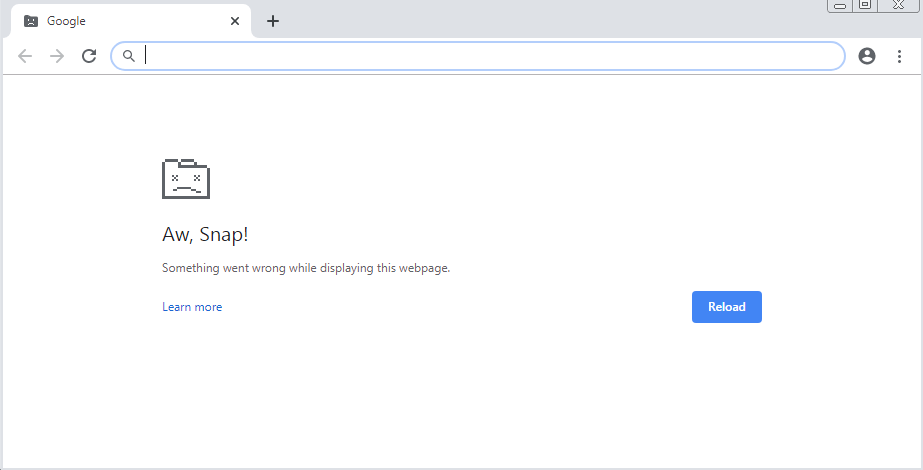
\includegraphics[width=\textwidth]{chrome_error}
    \caption{Ein Crash im Chrome-Browser}
  \end{subfigure}
  \hspace{0.5cm}
  \begin{subfigure}[b]{0.4\linewidth}
    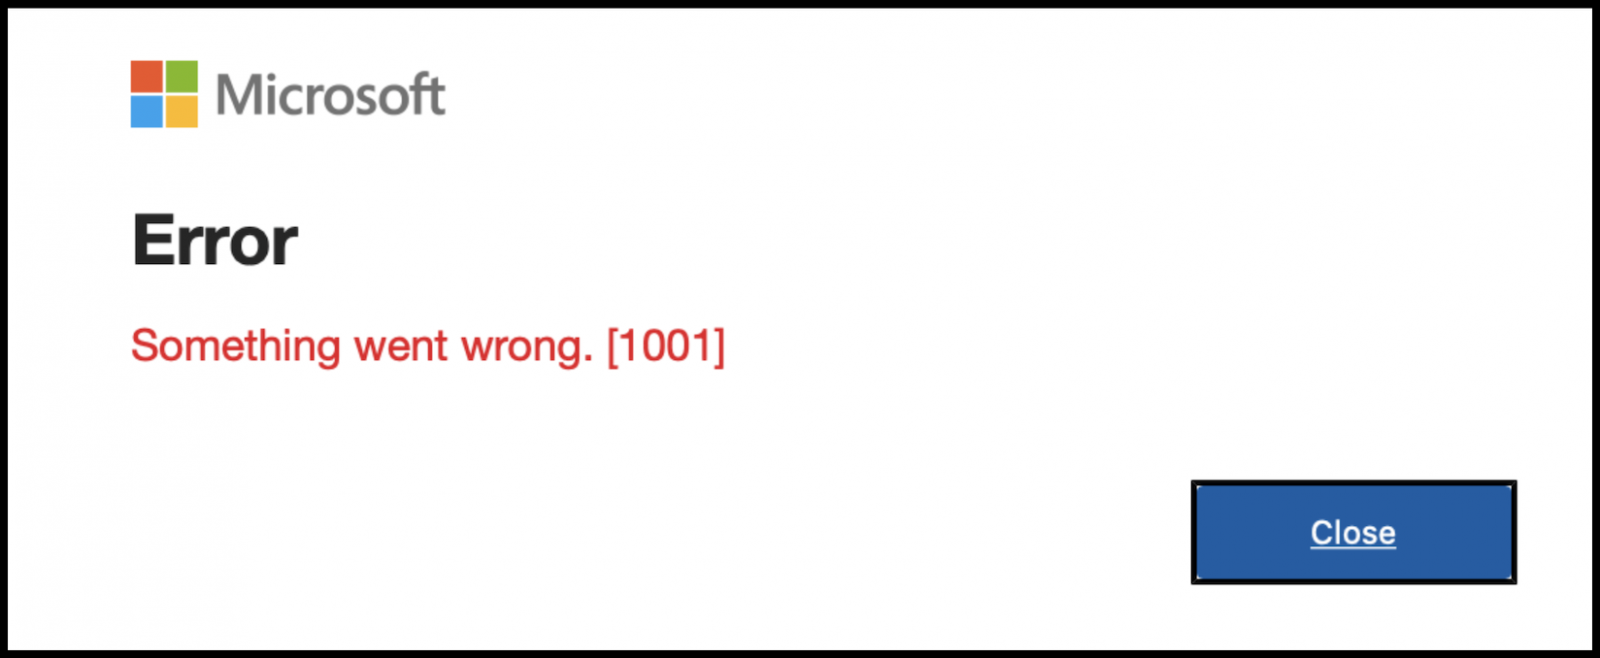
\includegraphics[width=\textwidth]{microsoft_error}
    \caption{Ein Fehler während des Microsoft Logins}
  \end{subfigure}
  \caption{Fehler in alltäglichen Anwendungen}
\end{figure}

Kaum eine Software is frei von Fehlern, welche je nach schwere ein großes Betriebsrisiko darstellen, weswegen die Vermeidung von diesen eine hohe Bedeutung
in der Entwicklung hat. 
Ein Ansatz, welcher in den letzen Jahren zunehmend an Bedeutung gewonnen hat sind stärkere Typsysteme, welche vermeintlich dafür sorgen, dass Fehler bereits
in der Entwicklung abgefangen werden können.
Beispiele für jüngere Entwicklungen in diesem Bereich sind Technologien wie TypeScript, welches versucht JavaScript zu typisieren, oder Rust, als eine Sprache die einen Fokus auf
ein ausdrucksstarkes Typsystem legt.

\begin{figure}[H]
  \centering
  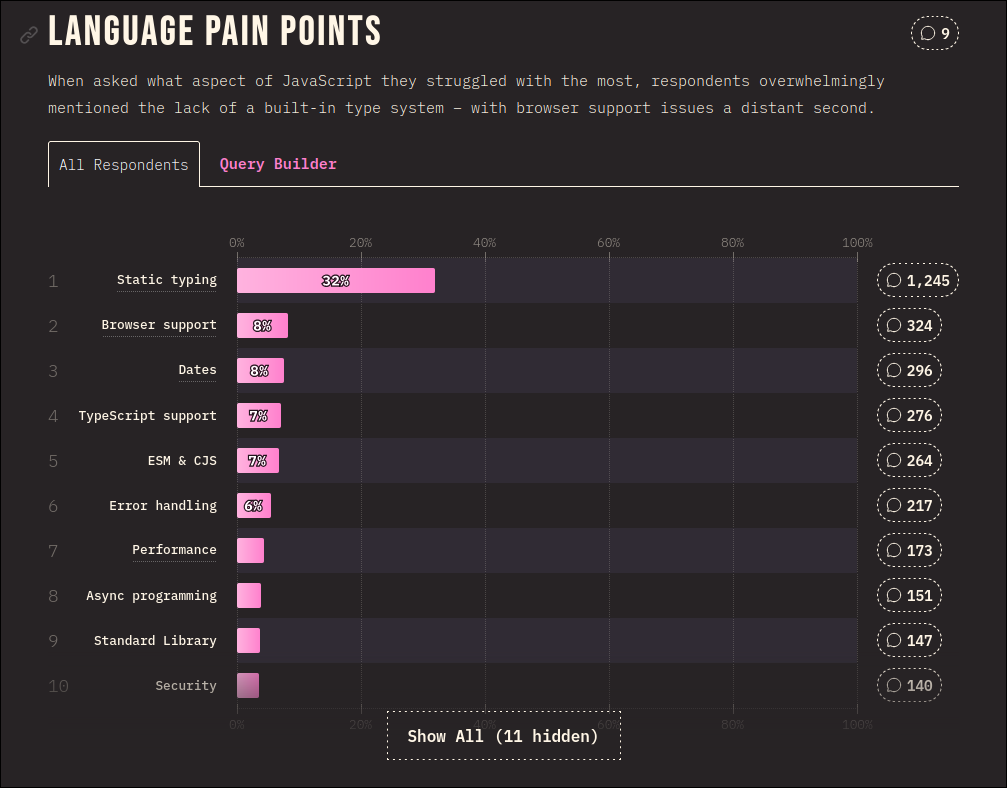
\includegraphics[width=0.9\textwidth]{state_of_js}
  \caption{32\% der Befragten in der \textquote{State of JavaScript 2024} Umfrage gaben an das (fehlende) statische Typisierung einer ihrer größten Probleme mit der Sprache sei \cite{Greif_Burel_2024}}
\end{figure}

\subsection{Ziel der Arbeit} 
Was hat der/die Leser*in von dieser Arbeit? Was soll er/sie nach dem Lesen gelernt haben?

Im folgenden sollen Eigenschaften und Vor- wie auch Nachteile von Typsystemen dargestellt werden, um aufzuzeigen 
